\documentclass[tikz,border=2pt]{standalone}
\usepackage{amsmath}
\usetikzlibrary{arrows.meta}
\begin{document}
% Player 1 moves twice: Stop/Continue at h, then (after Continue and r) a/b at h'. A pure strategy
% picks one action at each information set, so |S_1| = 2*2 = 4: (Stop,a), (Stop,b), (Continue,a),
% (Continue,b); the choice at h' is part of the plan even though Stop excludes h'. Player 2 has 2.
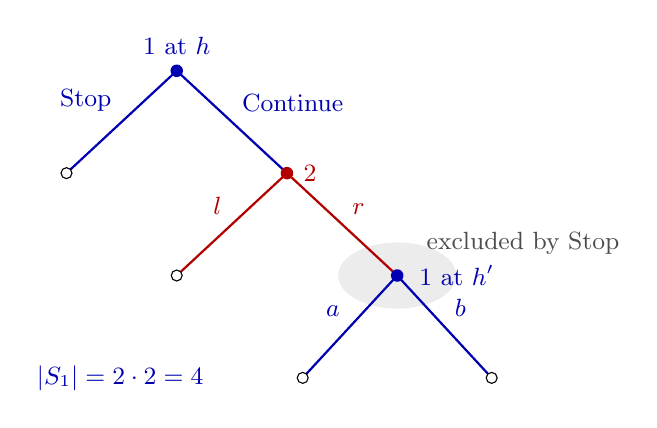
\begin{tikzpicture}[font=\small, >={Latex[length=2mm]},
    dec/.style={circle, fill, inner sep=1.6pt}, term/.style={circle, draw, fill=white, inner sep=1.4pt}]
  % node excluded by Stop
  \fill[gray!15] (2.8,-2.6) ellipse (0.75 and 0.42);
  % edges
  \draw[thick, blue!70!black] (0,0) -- node[above left, pos=0.5] {Stop} (-1.4,-1.3);
  \draw[thick, blue!70!black] (0,0) -- node[above right, pos=0.5] {Continue} (1.4,-1.3);
  \draw[thick, red!70!black] (1.4,-1.3) -- node[above left, pos=0.5] {$l$} (0,-2.6);
  \draw[thick, red!70!black] (1.4,-1.3) -- node[above right, pos=0.5] {$r$} (2.8,-2.6);
  \draw[thick, blue!70!black] (2.8,-2.6) -- node[above left, pos=0.5] {$a$} (1.6,-3.9);
  \draw[thick, blue!70!black] (2.8,-2.6) -- node[above right, pos=0.5] {$b$} (4.0,-3.9);
  % decision nodes
  \node[dec, blue!70!black, label={[blue!70!black]above:{$1$ at $h$}}] at (0,0) {};
  \node[dec, red!70!black, label={[red!70!black]right:$2$}] at (1.4,-1.3) {};
  \node[dec, blue!70!black, label={[blue!70!black, xshift=2pt]right:{$1$ at $h'$}}] at (2.8,-2.6) {};
  % terminal nodes
  \foreach \p in {(-1.4,-1.3), (0,-2.6), (1.6,-3.9), (4.0,-3.9)} \node[term] at \p {};
  \node[gray!60!black, anchor=south west] at (3.05,-2.45) {excluded by Stop};
  % strategy count
  \node[blue!70!black, anchor=west] at (-1.9,-3.9) {$|S_1|=2\cdot2=4$};
\end{tikzpicture}
\end{document}
